%----------------------------------------------------------------------------------------
%	PACKAGES AND DOCUMENT CONFIGURATIONS
%----------------------------------------------------------------------------------------

\documentclass{article}


\usepackage{graphicx} % Required for the inclusion of images
\usepackage{subcaption} % Required for the inclusion of images
\usepackage{natbib} % Required to change bibliography style to APA
\usepackage{amsmath} % Required for some math elements 
\usepackage{float}


\usepackage{xcolor}
\usepackage{listings}
\lstset{
    basicstyle=\footnotesize \ttfamily ,
	escapeinside=``,
	linewidth=\textwidth,
	numbers=left,
	numberstyle=\footnotesize  \ttfamily \color{blue},
	frame=trbl,
	aboveskip=1em,
	framextopmargin=2pt,framexbottommargin=2pt,abovecaptionskip=-3pt,belowcaptionskip=3pt,
} %Required for inserting code


%\usepackage{times} % Uncomment to use the Times New Roman font

%----------------------------------------------------------------------------------------
%	DOCUMENT INFORMATION
%----------------------------------------------------------------------------------------

\title{\textbf{Project 2:  Understanding Cache Memories}} % Title

\author{519021911045, Weihao Jiang, weihao.jiang@sjtu.edu.cn} % Author name and email

\date{\today} % Date for the report
\setlength{\parindent}{0pt}
\setlength{\parskip}{1ex}
\begin{document}

\maketitle % Insert the title, author and date

\section{Introduction}

In this project, we experimentally learn about the impact that cache memories can have on the performance of computer programming. The lab consists of two parts. In the first part,we write a  program that simulates the behavior of a cache memory. In the second part, we optimize a small matrix transpose function, with the goal of minimizing the number of cache misses.

After completing this project, we become more familiar with cache memories and computer architecture and have a keen insight into the interactions between algorithm and hardware that affect the performance of programs.

\section{Experiments}

\subsection{Part A}

\subsubsection{Analysis}

In Part A we write a cache simulator in \texttt{csim.c} that takes a valgrind memory trace as input, simulates the hit/miss behavior of a cache memory on the trace, and outputs the total number of hits, misses, and evictions.

The project has provided a reference cache simulator, which uses the LRU(least-recently used) replacement policy when choosing which cache line to evict. Our goal is to output the same result as this reference do and there's no need to simulate the actual memory read/write part. We have three values for interest: hit, miss and eviction.

Our jobs here is simple, by following the cache process. Perform a multi-way tag query. "hit" is increased if our data is in one of these ways. When the cache misses, we need to brought them from the main memory, and this increases the "miss" in our interest. When the cache is currently full, we maintain a counter that increases every query, and use this counter to mark the last used time. With LRU policy, we may get the victim and refresh it. This increases the "eviction" in our interest.

We may found that instructions like read or write would not affect the main process in our cache finding, but the modify needs to be specially treated. Modify can be presented as a read and write, while the write is always in cache (as just read it), we need to increase "hit" additionally to simulate this.

The code is short and intuitive, and shown in the next section.

\subsubsection{Code}
\begin{lstlisting}
#include "cachelab.h"
#include <stdio.h>
#include <getopt.h>
#include <stdlib.h>
#include <stdint.h>
#include <string.h>

typedef uint64_t addr_t;

#define MASK(high, low) ((((addr_t)1<<(high - low))-1)<<low)
#define BLOCK(addr, cfg) (addr & MASK((cfg).block,0))
#define SET(addr, cfg) \
    ((addr & MASK((cfg).block+(cfg).set,(cfg).block)) >> (cfg).block)
#define TAG(addr, cfg) (addr>> ((cfg).set+(cfg).block))

struct result {
    int hit;
    int miss;
    int evict;
};

struct configuration {
    int verbose;
    int set;
    int ways;
    int block;
    FILE *traceFile;
    struct result result;
};

/* Indexing the cache */

struct c_block {
    addr_t tag;
    int valid;
    int dirty;
    addr_t last_used;
};

typedef struct c_block c_block;
typedef c_block *c_set;
typedef c_set *c_way;
typedef c_way *cache;

#define for_each_way(wayptr, cache, cfg) \
    for(wayptr = cache; wayptr < cache + (cfg).ways; wayptr++)

#define for_each_set(setptr, way, cfg) \
    for(setptr = way; setptr < way + (1 << (cfg).set); setptr++)

#define for_each_block(blockptr, set, cfg) \
   for(blockptr = set; blockptr < set + (1 << (cfg).block); blockptr++)

void printHelpInfo () {
  printf ("Usage: ./csim [-hv] -s <s> -E <E> -b <b> -t <tracefile>\n");
  printf ("  -h: Optional help flag that prints usage info\n");
  printf ("  -v: Optional verbose flag that displays trace info\n");
  printf ("  -s <s>: "
        "Number of set index bits (S = 2^s is the number of sets)\n");
  printf ("  -E <E>: Associativity (number of lines per set)\n");
  printf ("  -b <b>: "
          "Number of block bits (B = 2^b is the block size)\n");
  printf ("  -t <tracefile>: Name of the valgrind trace to replay\n");
}

void 
  cacheOp (cache *c, 
           addr_t addr, int curr, struct configuration *cfg) {
  c_way *set;
  struct c_block *block = NULL;
  int hit = 0, cold = 0, last_used = curr;
  for_each_way(set, *c, *cfg) {
    if ((*set)[SET(addr, *cfg)]->tag == TAG(addr, *cfg)
        && (*set)[SET(addr, *cfg)]->valid) {
      hit = 1;
      block = (*set)[SET(addr, *cfg)];
      break;
    }
    if (cold)
      continue;
    if (!(*set)[SET(addr, *cfg)]->valid) {
      block = (*set)[SET(addr, *cfg)];
      cold = 1;
    }
    else if (last_used > (*set)[SET(addr, *cfg)]->last_used) {
      last_used = (*set)[SET(addr, *cfg)]->last_used;
      block = (*set)[SET(addr, *cfg)];
    }
  }
  block->last_used = curr;
  block->valid = 1;
  block->tag = TAG(addr, *cfg);
  if (hit) {
    cfg->result.hit++;
    if (cfg->verbose)
      printf ("S %lx hit\n", addr);
    return;
  }
  else {
    cfg->result.miss++;
    if (cold) {
      if (cfg->verbose)
        printf ("S %lx miss\n", addr);
      return;
    }
    else {
      cfg->result.evict++;
      if (cfg->verbose)
        printf ("S %lx evict\n", addr);
    }
  }
  return;
}

void sizeexpand (void (*action)
                        (cache *, addr_t, int, struct configuration *),
                 cache *c, addr_t addr, int curr, int size, int modify,
                 struct configuration *cfg) {
  int offset;
  for (offset = 0; offset < size; offset += (1 << cfg->block)) {
    action (c, (addr >> cfg->block << cfg->block) + offset, curr, cfg);
    if (modify)
      cfg->result.hit++;
  }
}

struct configuration optparse (int argc, char **argv) {
  struct configuration config;
  const char *optString = "hvs:E:b:t:";
  char opt = getopt (argc, argv, optString);
  config.verbose = 0;
  while (opt != -1) {
    switch (opt) {
      case 'h':
        printHelpInfo ();
        exit (0);
      case 'v':
        config.verbose = 1;
        break;
      case 's':
        config.set = atoi (optarg);
        if (config.set <= 0) {
          printf ("Error: set index bits.\n");
          exit (-1);
        }

        break;
      case 'E':
        config.ways = atoi (optarg);
        if (config.ways <= 0) {
          printf ("Error: associativity.\n");
          exit (-1);
        }
        break;
      case 'b':
        config.block = atoi (optarg);
        if (config.block <= 0) {
          printf ("Error: number of block bits.\n");
          exit (-1);
        }
        break;
      case 't':
        config.traceFile = fopen (optarg, "r");
        if (!config.traceFile) {
          printf ("Error: opening file\n");
          exit (-1);
        }
        break;
    }
    opt = getopt (argc, argv, optString);
  }
  return config;
}

int main (int argc, char **argv) {
  struct configuration cfg = optparse (argc, argv);
  memset (&cfg.result, 0, sizeof (struct result));

  cache c = malloc (cfg.ways * sizeof (c_way));
  c_way *wayptr;
  for_each_way(wayptr, c, cfg) {
    c_set *setptr;
    *wayptr = malloc ((1 << cfg.set) * sizeof (c_set));
    for_each_set(setptr, *wayptr, cfg) {
      *setptr = malloc ((1 << cfg.block) * sizeof (c_block));
      memset (*setptr, 0, (1 << cfg.block) * sizeof (c_block));
    }
  }
  char inst, tmp;
  addr_t addr;
  int size, curr = 0;

  while (fscanf (cfg.traceFile, "%c%lx%c%d", &inst, &addr, &tmp, &size)
         != EOF) {
    if (inst == 'S' || inst == 'L')
      sizeexpand (cacheOp, &c, addr, curr, size, 0, &cfg);
    else if (inst == 'M')
      sizeexpand (cacheOp, &c, addr, curr, size, 1, &cfg);
    curr++;
  }
  printSummary (cfg.result.hit, cfg.result.miss, cfg.result.evict);
  return 0;
}
\end{lstlisting}


\subsubsection{Evaluation}

The correctness is shown in the fig \ref{fig:evalA}.

\begin{figure}
    \centering
    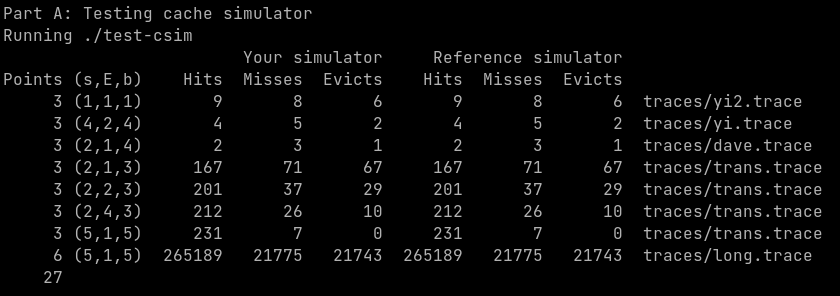
\includegraphics[width=0.95\textwidth]{1.png}
    \caption{Evaluation of part A}
    \label{fig:evalA}
\end{figure}

\subsection{Part B}

\subsubsection{Analysis}

To optimize matrix transpose we should know that locality plays a core part in cache miss optimization. To increase the locality, the first thing comes to our mind would be partitioning. By separating the whole matrix into small parts, we will keep our read cache and reduce the cache miss.

What's the step we do the partitioning? Let's take 32x32 matrix as an example: the $A[i][j]$ will take the same cache place as $A[i+8][j]$, and separating it into 4 8x8 matrices would be fine, and the result passes the test.

A 61x67 matrix, would be difficult to analyse. As matrices are actually stored as a long list, a 67 per line matrix actually provides a pretty good cache performance: they will not be easily overlapped. With an iteration to decide how to separate it, we found the top-9 step can all pass the test.

\begin{table}[H]
    \centering
    \begin{tabular}{c|ccccccccc}
    \hline
    Step & 23   & 17   & 21   & 18   & 22   & 19   & 16   & 14   & 20   \\ \hline
    Miss & 1922 & 1944 & 1950 & 1954 & 1954 & 1972 & 1986 & 1990 & 1995 \\ \hline
    \end{tabular}
    \end{table}

However, the 64x64 matrix would be the worst one to be presented to the cache, as $A[i][j]$ will take the same cache place as $A[i+4][j]$, and transposing 4x4 matrices may not be a good idea - they are too small to elevate the performance.

We find that for each 32 cache, with only 4 lines cacheable, we may utilize the cache as 4x8, which have an extra of 4x4 blocks. We may copy a 4x8 every time (which would be out of order), and arrange them in the same block to increase locality. See fig. \ref{fig:same} for illustration.

\begin{figure}[H]
    \centering
    \begin{subfigure}{.2\textwidth}
      \centering
      % include first image
      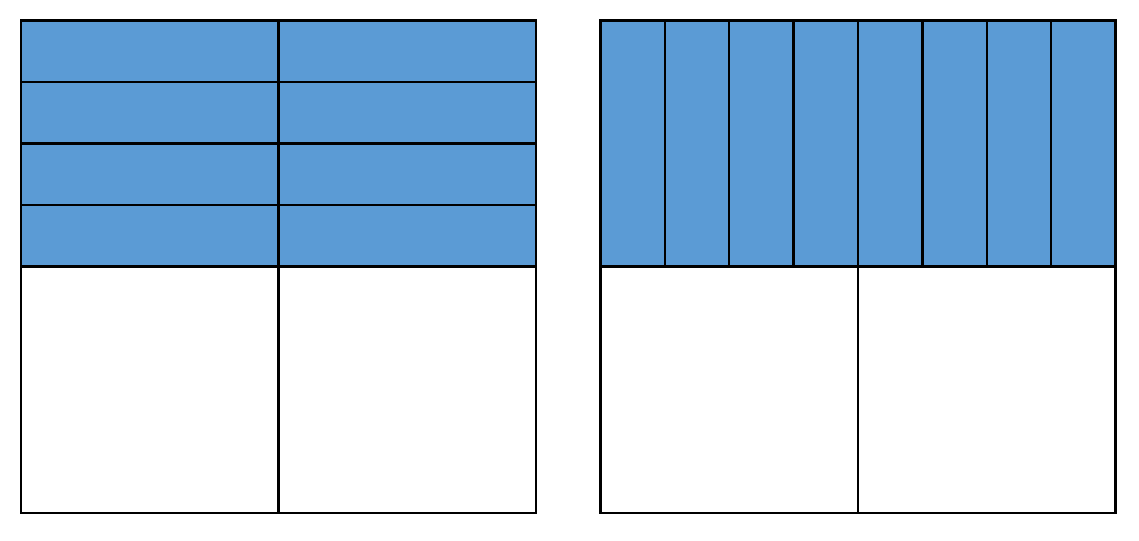
\includegraphics[width=\textwidth]{2.png}
      \caption{Step 1}
    \end{subfigure}
    \begin{subfigure}{.2\textwidth}
      \centering
      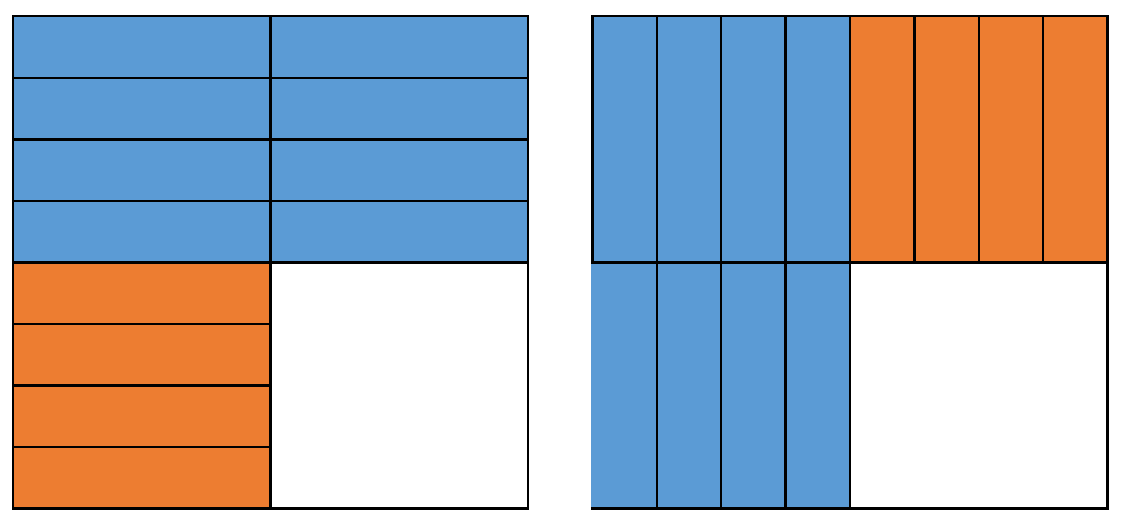
\includegraphics[width=\textwidth]{3.png}
      \caption{Step 2}
    \end{subfigure}
    \newline
    \centering
    \begin{subfigure}{.2\textwidth}
      \centering
      % include first image
      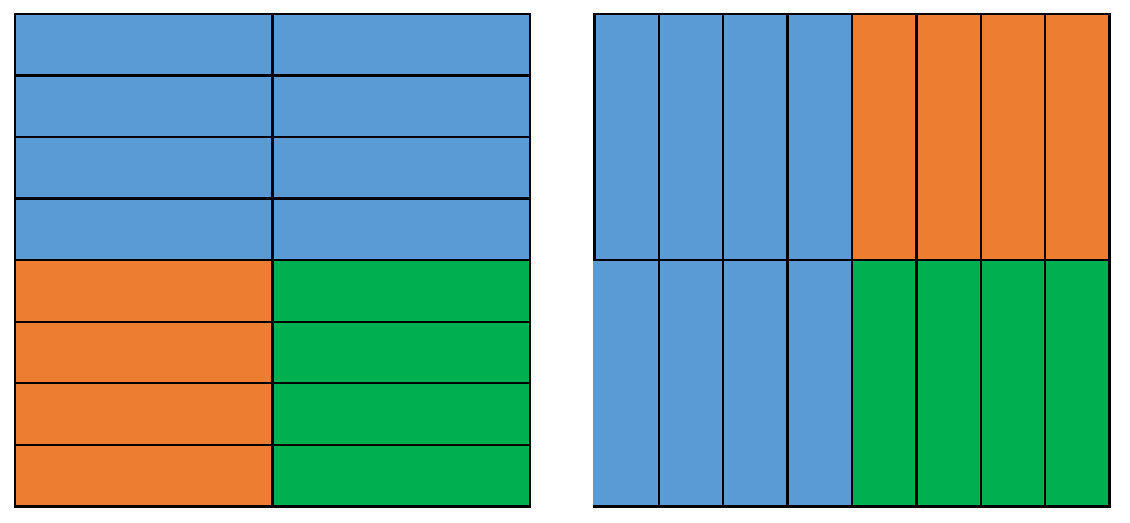
\includegraphics[width=\textwidth]{4.png}
      \caption{Step 3}
    \end{subfigure}
    \caption{Arrange method}
    \label{fig:same}
    \end{figure}

\subsubsection{Code}

\begin{lstlisting}
   /* Skip the provided part*/

#define PARTITION(length) \
    for (ia = 0; ia < N; ia += length) \
    for (ja = 0; ja < M; ja += length) \
    for (ib = ia; ib < ia + length && ib < N; ib++) { \
    for (jb = ja; jb < ja + length && jb < M; jb++)
  
  char transpose_submit_desc[] = "Transpose submission";
  void trans (int M, int N, int A[N][M], int B[M][N]);
  void transpose_submit (int M, int N, int A[N][M], int B[M][N]) {
    int ia, ja, ib, jb;
    int temp1, temp2, temp3, temp4, temp5, temp6, temp7, temp8;
    switch (M) {
      case 32:
        PARTITION(8) {
                if (ib != jb)
                  B[jb + 0][ib + 0] = A[ib + 0][jb + 0];
                else {
                  temp1 = A[ib + 0][jb + 0];
                  temp2 = ib;
                }
              }
              if (ia == ja)
                B[temp2][temp2] = temp1;
            }
        break;
      case 61:
        PARTITION(23) {
                if (ib != jb)
                  B[jb + 0][ib + 0] = A[ib + 0][jb + 0];
                else {
                  temp1 = A[ib + 0][jb + 0];
                  temp2 = ib;
                }
              }
              if (ia == ja)
                B[temp2][temp2] = temp1;
            }
        break;
      case 64:
        for (ia = 0; ia < M; ia += 8) {
          for (ja = 0; ja < M; ja += 8) {
            for (ib = ia; ib < ia + 4; ib++) {
              temp1 = A[ib + 0][ja + 0];
              temp2 = A[ib + 0][ja + 1];
              temp3 = A[ib + 0][ja + 2];
              temp4 = A[ib + 0][ja + 3];
              temp5 = A[ib + 0][ja + 4];
              temp6 = A[ib + 0][ja + 5];
              temp7 = A[ib + 0][ja + 6];
              temp8 = A[ib + 0][ja + 7];
              B[ja + 0][ib + 0] = temp1;
              B[ja + 0][ib + 4] = temp5;
              B[ja + 1][ib + 0] = temp2;
              B[ja + 1][ib + 4] = temp6;
              B[ja + 2][ib + 0] = temp3;
              B[ja + 2][ib + 4] = temp7;
              B[ja + 3][ib + 0] = temp4;
              B[ja + 3][ib + 4] = temp8;
            }
            for (jb = ja; jb < ja + 4; jb++) {
              temp5 = A[ia + 4][jb + 0];
              temp6 = A[ia + 5][jb + 0];
              temp7 = A[ia + 6][jb + 0];
              temp8 = A[ia + 7][jb + 0];
              temp1 = B[jb + 0][ia + 4];
              temp2 = B[jb + 0][ia + 5];
              temp3 = B[jb + 0][ia + 6];
              temp4 = B[jb + 0][ia + 7];
              B[jb + 0][ia + 4] = temp5;
              B[jb + 0][ia + 5] = temp6;
              B[jb + 0][ia + 6] = temp7;
              B[jb + 0][ia + 7] = temp8;
              B[jb + 4][ia + 0] = temp1;
              B[jb + 4][ia + 1] = temp2;
              B[jb + 4][ia + 2] = temp3;
              B[jb + 4][ia + 3] = temp4;
            }
            for (jb = ja + 4; jb < ja + 8; jb++) {
              temp1 = A[ia + 4][jb + 0];
              temp2 = A[ia + 5][jb + 0];
              temp3 = A[ia + 6][jb + 0];
              temp4 = A[ia + 7][jb + 0];
              B[jb + 0][ia + 4] = temp1;
              B[jb + 0][ia + 5] = temp2;
              B[jb + 0][ia + 6] = temp3;
              B[jb + 0][ia + 7] = temp4;
            }
          }
        }
        break;
      default:
        trans (M, N, A, B);
    }
  }
  
\end{lstlisting}

\subsubsection{Evaluation}

The correctness is shown in the fig \ref{fig:evalB}. This also contains the summary part, which is the evaluation of A and B.

\begin{figure}[H]
    \centering
    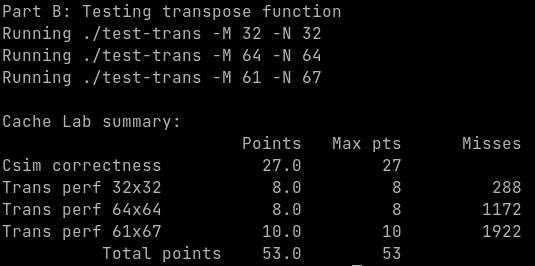
\includegraphics[width=0.8\textwidth]{5.png}
    \caption{Evaluation of part B}
    \label{fig:evalB}
\end{figure}

\section{Conclusion}

\subsection{Problems}

\begin{itemize}
	\item \textbf{Part A}
	
    The main obstacle for this part is to find a good data structure to for better indexing. At first we used a plain large array to store all thing and manage them by pointer arithmetics. However this becomes a painful debugging issues, with \texttt{SIGSEGV} being around the whole program. After changing the structure using C's struct, the programming is more intuitive and easy to debug. Pointers are not so easy to handle, and it's critical to use tools to handle them.
		
	\item \textbf{Part B}
	
    The main obstacle for this part is to find a smart way to handle with cache miss. At first we just trying hard on trivial partitioning. Running the test costs a lot of time, and we even wrote a python script to iterate all posible partitioning steps! After getting back onto the cache itself, and understanding that the cache could be a rectangle-shaped matrix, the problem is getting solved.
\end{itemize}

\subsection{Achievements}

First, we are more familiar with computer architecture and cache optimization after writing the cache simulator and optimizing matrix transposing with our own hands. What's more, the process of optimizing in Part B also brought us a keen appreciation for the cache performance, which is critical to the performance of programs nowaday. Though complex compilers are doing these things for us, and there're much more talented cache utilizing techniques among them, we could learn from it and organize our code to be more efficient.

Second, it is relatively excited to pass the 64x64 matrix after careful design of logic and implementation. Meanwhile, though utilizing tools to decide arguments didn't help in this experiment, our ability facing problems still gets exercised.

Finally, we would like to specially thank Miss Shen and TAs for their kind and patient support. And we are also grateful to Shanghai Jiao Tong University and School of Electronic Information and Electrical Engineering to provide such a valuable and interesting course.



%----------------------------------------------------------------------------------------


\end{document}